\documentclass{beamer}
\usepackage{tikz}
% Force exact PDF slide size
\usepackage{geometry}
\geometry{paperwidth=35cm,paperheight=14cm} % ~1328x531px @ 96dpi
\usepackage{xcolor}
\usetheme{default}
\setbeamertemplate{navigation symbols}{}   % <-- Hides bottom-right symbols
\usepackage{graphicx}
\usepackage[most]{tcolorbox} % powerful box package
\usetikzlibrary{arrows.meta}
\usetikzlibrary{shapes,positioning}
\usepackage{subcaption}
\begin{document}
	
\begin{frame}
\begin{columns}[T]	
	% Column 1
	\begin{column}{0.31\textwidth}
		{\Large\textbf{ \textcolor{red}{Closed-form} DSM method for the free vibration of orthotropic rectangular thin plates}}\par\vspace{0.4em}
		
		% Create a box around the equations
		\fbox{%
			\scalebox{0.8}{%
				\begin{minipage}{1.2\linewidth}
					\centering
					\textbf{Four SOV-type eigenvalue equations}\par\vspace{0.3em}
					\begin{align*}
						\alpha_1 &= \chi \sqrt{\sqrt{\left(\frac{D_{12}I_2}{D_{11}I_1}-2\frac{D_{66}I_3}{D_{11}I_1}\right)^2 
								- \frac{D_{22}I_4}{D_{11}I_1} + b^4\Omega_x^4} 
							+ \frac{D_{12}I_2}{D_{11}I_1} - 2\frac{D_{66}I_3}{D_{11}I_1}}\\[0.3em]
						\beta_1 &= \chi \sqrt{\sqrt{\left(\frac{D_{12}I_2}{D_{11}I_1}-2\frac{D_{66}I_3}{D_{11}I_1}\right)^2 
								- \frac{D_{22}I_4}{D_{11}I_1} + b^4\Omega_x^4} 
							- \frac{D_{12}I_2}{D_{11}I_1} + 2\frac{D_{66}I_3}{D_{11}I_1}}\\
						\alpha_2 &= \frac{1}{\chi} \sqrt{ \sqrt{ \left( \frac{D_{12}J_2}{D_{22}J_1} - 2\frac{D_{66}J_3}{D_{22}J_1} \right)^2 
								- \frac{D_{11}J_4}{D_{22}J_1} + \frac{a^4 D_{11}}{D_{22}} \Omega_y^4 } 
							+ \frac{D_{12}J_2}{D_{22}J_1} - 2 \frac{D_{66}J_3}{D_{22}J_1}}\\[0.3em]
						\beta_2 &= \frac{1}{\chi} \sqrt{ \sqrt{ \left( \frac{D_{12}J_2}{D_{22}J_1} - 2 \frac{D_{66}J_3}{D_{22}J_1} \right)^2 
								- \frac{D_{11}J_4}{D_{22}J_1} + \frac{a^4 D_{11}}{D_{22}} \Omega_y^4 } 
							- \frac{D_{12}J_2}{D_{22}J_1} + 2 \frac{D_{66}J_3}{D_{22}J_1}}
					\end{align*}
				\end{minipage}
			}%
		} % end fbox
		
		\vspace{0.5em}
		\centering {\Huge \textbf{+}}\vspace{0.5em}
		\tikz[remember picture] \node (node1) {}; % <--- mark start node
		% Create a box around the equations
		\fbox{%
			\scalebox{0.8}{%
				\begin{minipage}{1.2\linewidth}
					\centering
					\textbf{Two eigenvalue equations from boundary condition}\par\vspace{0.5em}
					
					% Two-column layout inside the box
					\begin{minipage}{0.66\linewidth}
						\centering
						\centering
						\resizebox{0.8\textwidth}{!}{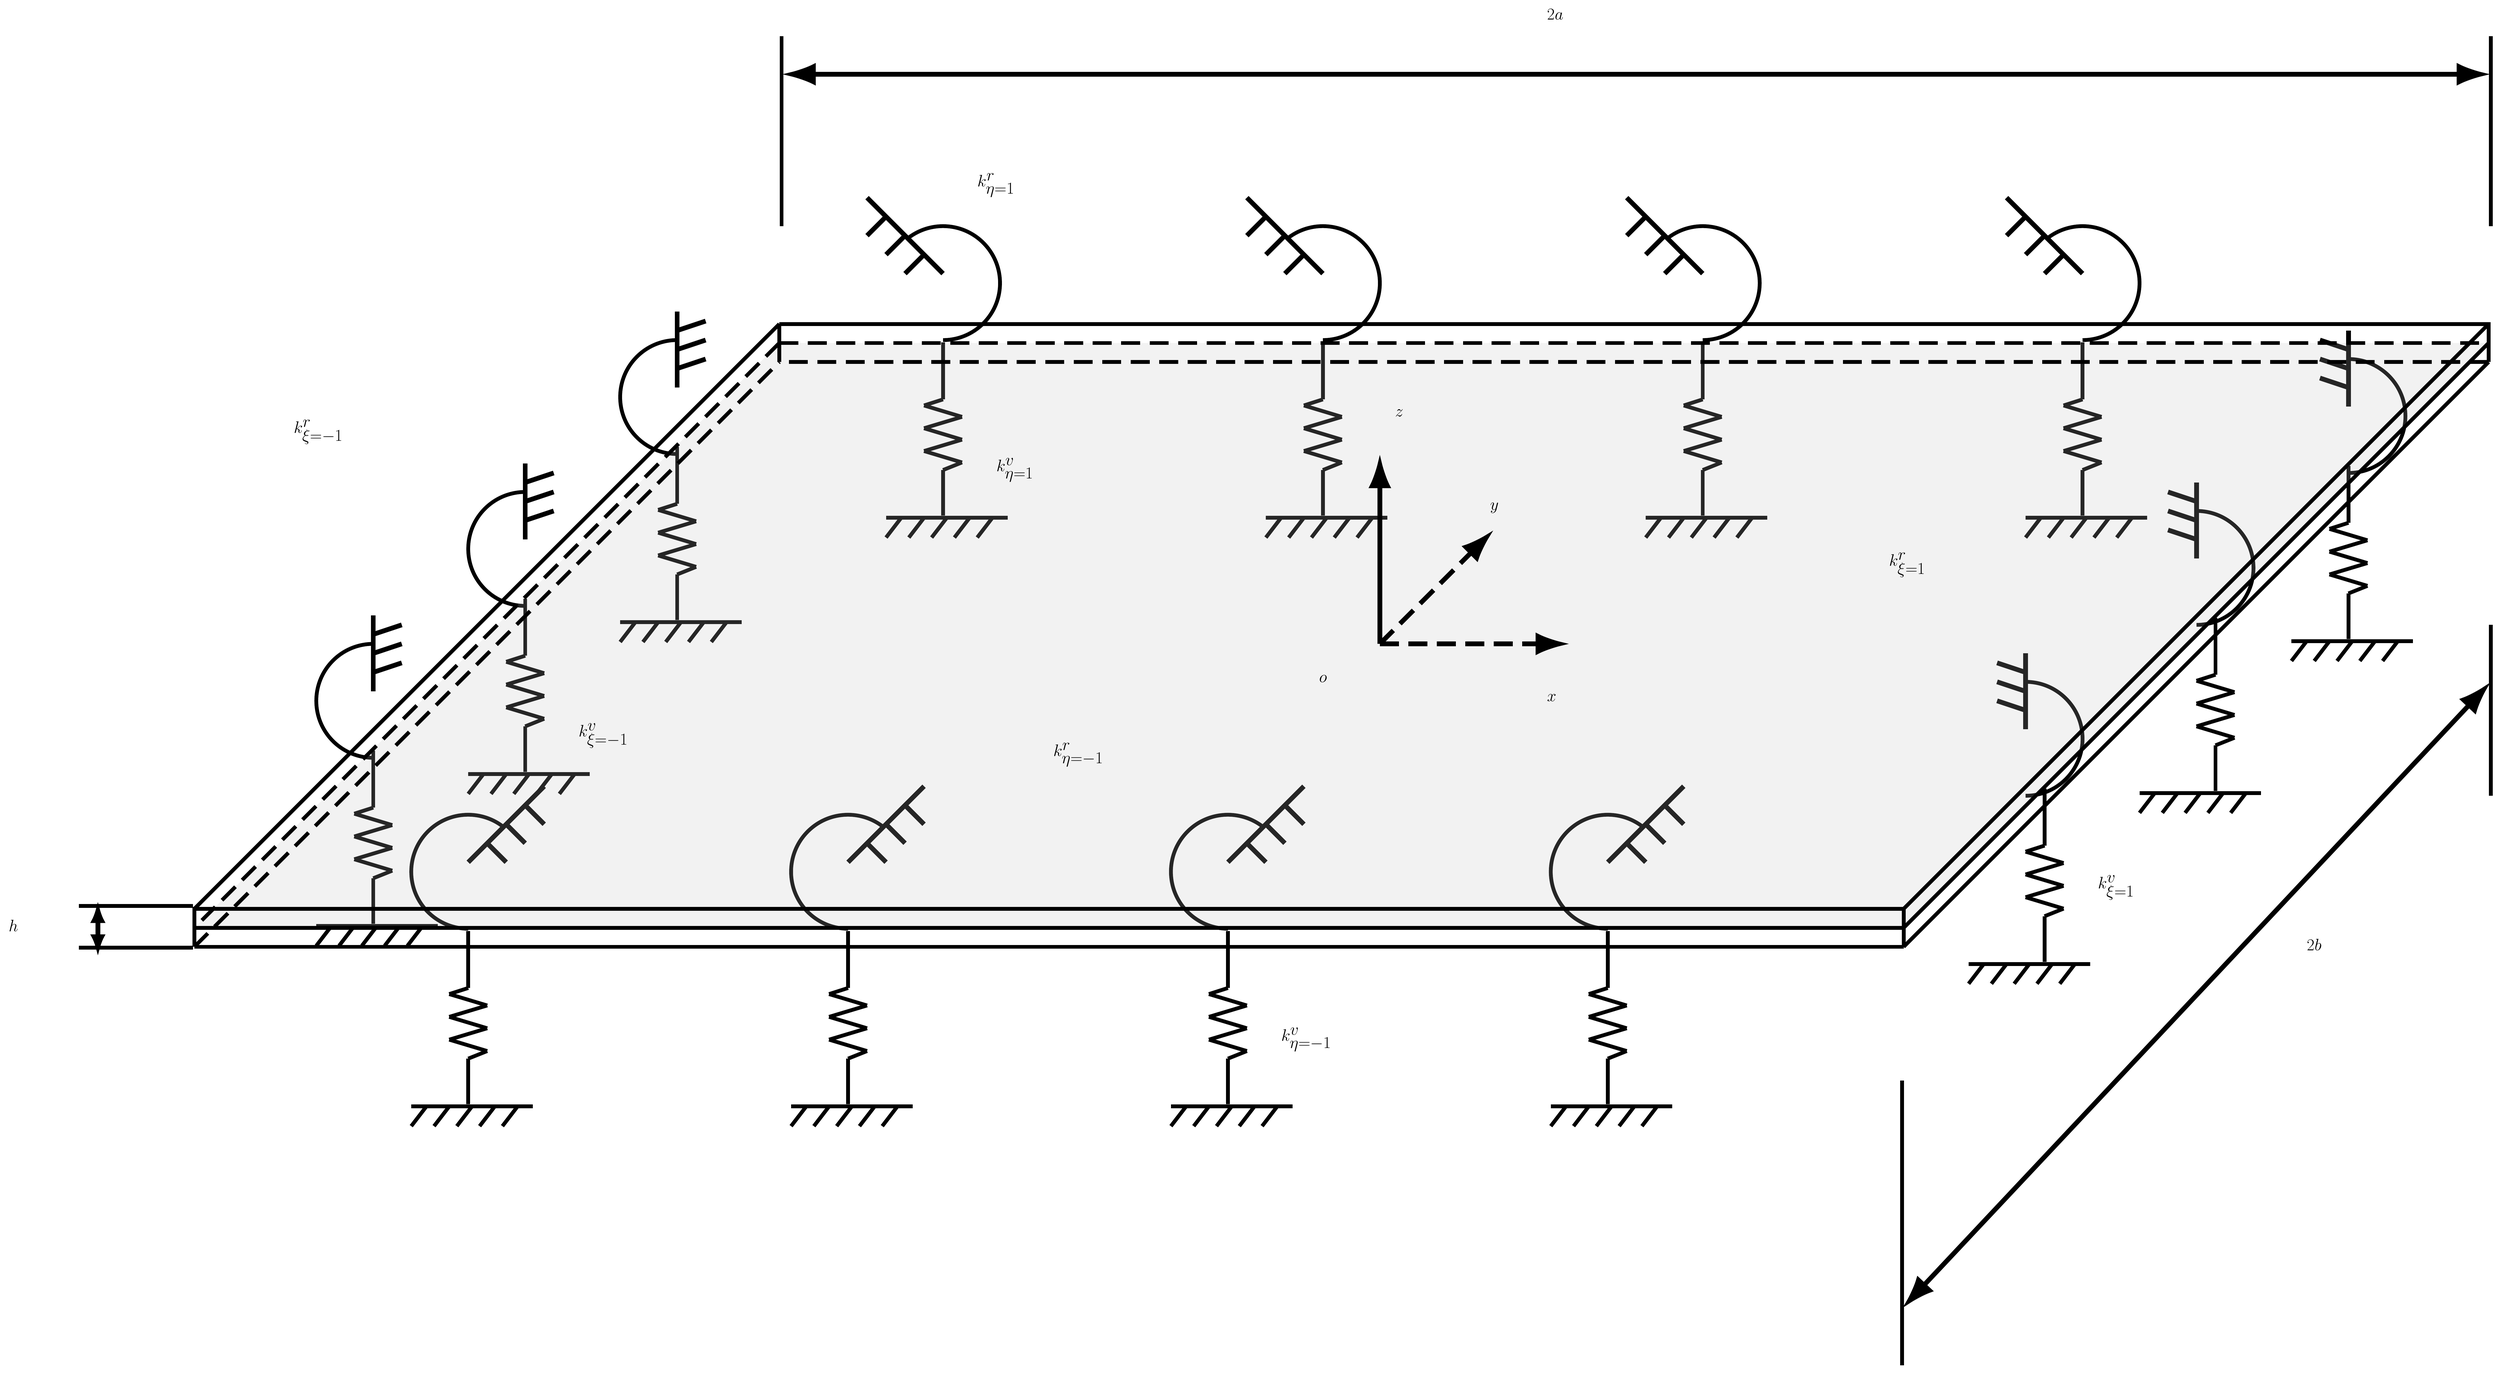
\begin{tikzpicture}[yscale=1]
	\tikzset{
	pics/boundary-box/.style={
		code={
			\begin{scope}[shift={(0mm,0mm)}]
				\definecolor{fc}{RGB}{204,204,204}
				\draw [fill=none, draw=black, line width=0.6mm] (000.0mm,0.0mm)
				-- ++(0.0mm,60.0mm)
				-- ++(-60.0mm,0.0mm)
				-- ++(0.0mm,-60.0mm)  % Adjusted the vertical length to 20mm
				-- ++(60.0mm,0.0mm)  % Adjusted the vertical length to 20mm
				-- cycle;
				\node [black, anchor=west, font=\fontsize{100}{0}\selectfont\bfseries] at (-40mm, 30mm) { $\textbf{?}$ };
			\end{scope}
		}
	}
}
\tikzset{
	pics/Mass-circle/.style={
		code={
			\draw[fill=gray!30, draw=black, line width=0.6mm] (0mm, 0mm) circle [radius=38mm];
		}
	}
}
\tikzset{
	pics/Beam/.style={
		code={\draw [fill=none,draw=black,line width=10.0mm] (000.0mm,0.mm)
			-- ++(600.0mm,0.0mm)
			;
			%% curvature
			\draw[fill=none, draw=gray, line width=4.0mm, dash pattern=on 20pt off 20pt] (000.0mm,0.mm) .. controls (200mm,-100mm) and (300mm,-50mm) .. (600.0mm,0mm);
			
			
		}
	}
}
\tikzset{
	pics/Spring-damp/.style={
		code={\begin{scope}[cm={0.4,0,0,0.4,(40.0mm,0mm)}]
				\draw [fill=none,draw=black,line width=2.0mm] (145.0mm,707.4mm)
				-- ++(0.0mm,33.0mm)
				;
				\draw [fill=none,draw=black,line width=2.0mm] (120.0mm,867.4mm)
				-- ++(50.0mm,-15.0mm)
				;
				\draw [fill=none,draw=black,line width=2.0mm] (170.0mm,852.4mm)
				-- ++(-50.0mm,-15.0mm)
				;
				\draw [fill=none,draw=black,line width=2.0mm] (120.0mm,837.4mm)
				-- ++(50.0mm,-15.0mm)
				;
				\draw [fill=none,draw=black,line width=2.0mm] (170.0mm,822.4mm)
				-- ++(-50.0mm,-15.0mm)
				;
				
				\draw [fill=none,draw=black,line width=2.0mm] (120.0mm,807.4mm)
				-- ++(50.0mm,-15.0mm)
				;
				
				\draw [fill=none,draw=black,line width=2.0mm] (170.0mm,792.4mm)
				-- (120.0mm,777.4mm)
				;
				
				\draw [fill=none,draw=black,line width=2.0mm] (120.0mm,777.4mm)
				-- ++(50.0mm,-15.0mm)
				;
				
				\draw [fill=none,draw=black,line width=2.0mm] (170.0mm,762.4mm)
				-- ++(-50.0mm,-15.0mm)
				;
				
				\draw [fill=none,draw=black,line width=2.0mm] (145.0mm,875.4mm)
				-- ++(-25.0mm,-8.0mm)
				;
				
				\draw [fill=none,draw=black,line width=2.0mm] (120.0mm,747.4mm)
				-- ++(25.0mm,-7.0mm)
				;
				
				\draw [fill=none,draw=black,line width=2.0mm] (145.0mm,875.4mm)
				-- (145.0mm,907.4mm)
				;
			\end{scope}
			% horizontal line above mass left
			\draw [fill=none,draw=black,line width=2.0mm] (58.0mm,363mm)
			-- ++(40.0mm,0.0mm)
			;
			
			%% damping left
			\begin{scope}[cm={0.4,0,0,-0.4,(0.0mm,645.9mm)}]
				\draw [fill=none,draw=black,line width=2.0mm] (115.0mm,827.7mm)
				-- ++(0.0mm,-35.3mm)
				-- (175.0mm,792.4mm)
				-- ++(0.0mm,35.0mm)
				;
				
				\draw [fill=none,draw=black,line width=2.0mm] (145.0mm,707.4mm)
				-- ++(0.0mm,85.0mm)
				;
				
				\draw [fill=none,draw=black,line width=2.0mm] (123.0mm,807.4mm)
				-- ++(44.0mm,0.0mm)
				;
				
				\draw [fill=none,draw=black,line width=2.0mm] (145.0mm,807.4mm)
				-- ++(0.0mm,100.0mm)
				;
			\end{scope}
			
			%% suspension arrow left
			\draw [fill=none,draw=black,line width=2.0mm] (58.0mm,283.4mm)
			-- ++(40.0mm,0.0mm)
			;
			\draw [fill=none,draw=black,line width=2.0mm] (78.0mm,363.4mm)
			-- ++(0mm,27.0mm)
			;
			%% vertical line upp
			\draw [fill=none,draw=black,line width=2.0mm] (78.0mm,283.4mm)
			-- ++(0.0mm,-30.0mm)
			;
		}
	}
}
\tikzset{
	pics/beam-Spring/.style={
		code={\begin{scope}[cm={0.4,0,0,0.4,(-38.0mm,-256.4mm)}]
				\draw [fill=none,draw=black,line width=2.0mm] (145.0mm,782.4mm)
				-- ++(0.0mm,-60.0mm)
				;
				\draw [fill=none,draw=black,line width=2.0mm] (120.0mm,867.4mm)
				-- ++(50.0mm,-15.0mm)
				;
				\draw [fill=none,draw=black,line width=2.0mm] (170.0mm,852.4mm)
				-- ++(-50.0mm,-15.0mm)
				;
				\draw [fill=none,draw=black,line width=2.0mm] (120.0mm,837.4mm)
				-- ++(50.0mm,-15.0mm)
				;
				\draw [fill=none,draw=black,line width=2.0mm] (170.0mm,822.4mm)
				-- ++(-50.0mm,-15.0mm)
				;
				\draw [fill=none,draw=black,line width=2.0mm] (120.0mm,807.4mm)
				-- ++(50.0mm,-15.0mm)
				;
				\draw [fill=none,draw=black,line width=2.0mm] (170.0mm,792.4mm)
				-- (145.0mm,782.4mm)
				;
				
				
			
				\draw [fill=none,draw=black,line width=2.0mm] (145.0mm,875.4mm)
				-- ++(-25.0mm,-8.0mm)
				;
				
				\draw [fill=none,draw=black,line width=2.0mm] (145.0mm,875.4mm)
				-- (145.0mm,950.4mm)
				;
			\end{scope}
			
		}
	}
}
\tikzset{
	pics/beam-arrow/.style={
		code={% bridge curve property 
			\draw [fill=none,draw=black,line width=2.0mm] (380.0mm,32.0mm)
			.. controls ++(85.0mm,-8.0mm) and ++(-60.0mm,-6.0mm) .. ++(135.0mm,-32.0mm)
			;
			%% arraw of bridge curve property 
			\draw [->, black, line width=6mm, >=stealth, shorten >=1pt] (515.0mm,0mm) -- ++(0.5,0); % Draws the arrowhead separately
			
		}
	}
}
\tikzset{
	pics/beam-prop-arrow/.style={
		code={% bridge curve deflection yx
			\draw [fill=none,draw=black,line width=2.0mm] (440.0mm,0.0mm)
			.. controls ++(85.0mm,5.0mm) and ++(-60.0mm,4.0mm) .. ++(135.0mm,36.0mm)
			;
			%% arraw of bridge curve deflection yx
			\draw [black, line width=2mm] (570.0mm,36.0mm) -- (580.0mm,36.0mm);
			\draw [->, black, line width=6mm, >=stealth, shorten >=1pt] (580.0mm,36.0mm) -- ++(0.5,0); % Draws the arrowhead separately
			
		}
	}
}
\tikzset{
	pics/mass-defle/.style={
		code={%% arraw of vehicle deflection yv 
			\draw [->,fill=none,draw=black,line width=2.50mm] (0.0mm,25.0mm)
			-- (30.0mm,25.0mm)
			-- (30.0mm,65.3mm)
			;			
		}
	}
}
\tikzset{
	pics/floor/.style={
		code={
			%  left
			\begin{scope}[cm={0.4,0,0,-0.4,(-42.0mm,377.0mm)}]
				\draw [fill=none,draw=black,line width=2.0mm] (30.0mm,939mm)
				-- (190.0mm,939mm)
				;
				\draw [fill=none,draw=black,line width=2.0mm] (50.0mm,939mm)
				-- (30.0mm,965mm)
				;
				\draw [fill=none,draw=black,line width=2.0mm] (80.0mm,939mm)
				-- (60.0mm,965mm)
				;
				\draw [fill=none,draw=black,line width=2.0mm] (110.0mm,939mm)
				-- (90.0mm,965mm)
				;
				\draw [fill=none,draw=black,line width=2.0mm] (140.0mm,939mm)
				-- (120.0mm,965mm)
				;
				\draw [fill=none,draw=black,line width=2.0mm] (170.0mm,939mm)
				-- (150.0mm,965mm)
				;
			\end{scope}
			
		}
	}
}
\tikzset{
	pics/beam-rotation/.style={
		code={
			%%% arc representing rotation or deflection
			\draw [-,fill=none,draw=black,line width=2.00mm] 
			(0.0mm,25.0mm) arc [start angle=270, end angle=90, radius=30mm];
			\draw [fill=none,draw=black,line width=2.5mm] (0.0mm,60mm)
			-- (0.0mm,100mm)
			;
			
			\draw [fill=none,draw=black,line width=2.5mm] (0.0mm,70mm)
			-- (15.0mm,75mm)
			;
			\draw [fill=none,draw=black,line width=2.5mm] (0.0mm,80mm)
			-- (15.0mm,85mm)
			;
			\draw [fill=none,draw=black,line width=2.5mm] (0.0mm,90mm)
			-- (15.0mm,95mm)
			;
			
		}
	}
}
\tikzset{
	pics/beam-rotation-bot/.style={
		code={
			%%% arc representing rotation or deflection
			\draw [-,fill=none,draw=black,line width=2.00mm] 
			(0.0mm,25.0mm) arc [start angle=270, end angle=50, radius=30mm];
			\draw [fill=none,draw=black,line width=2.5mm] (0.0mm,60mm)
			-- (40.0mm,100mm)
			;
			
			\draw [fill=none,draw=black,line width=2.5mm] (10mm,70mm)
			-- (20.0mm,60mm)
			;
			\draw [fill=none,draw=black,line width=2.5mm] (20mm,80mm)
			-- (30.0mm,70mm)
			;
			\draw [fill=none,draw=black,line width=2.5mm] (30mm,90mm)
			-- (40.0mm,80mm)
			;
			
		}
	}
}
\tikzset{
	pics/Rectangular-Plate/.style={
		code={
			% Define the vertices of the rectangular plate
			\coordinate (A) at (0, 1, 0);
			\coordinate (B) at (90, 1, 0);
			\coordinate (C) at (90, 2, 0);
			\coordinate (D) at (0, 2, 0);
			\coordinate (A') at (0, 1, 80);
			\coordinate (B') at (90, 1, 80);
			\coordinate (C') at (90, 2, 80);
			\coordinate (D') at (0, 2, 80);
			\coordinate (E) at (0, 0, 0);
			\coordinate (F) at (90, 0, 0);
			\coordinate (E') at (0, 0, 80);
			\coordinate (F') at (90, 0, 80);
			
			% Fill the surface AA'B'B with gray and transparent
			\fill[gray!50, fill opacity=0.2] (A) -- (A') -- (B') -- (B) -- cycle;
			
			% Draw the edges of the bottom face
			\draw[black, line width=2mm, dashed, dash pattern=on 10mm off 5mm] (A) -- (B); % AB dashed
			\draw[black, line width=2mm] (B) -- (C) -- (D); % Remaining edges solid
			\draw[black, line width=2mm, dashed, dash pattern=on 10mm off 5mm] (D) -- (A); % AD dashed
			\draw[black, line width=2mm, dashed, dash pattern=on 10mm off 5mm] (A) -- (E); % AB dashed
			\draw[black, line width=2mm, dashed, dash pattern=on 10mm off 5mm] (F) -- (E); % AB dashed
			\draw[black, line width=2mm, dashed, dash pattern=on 10mm off 5mm] (F) -- (B); % AB dashed
			\draw[black, line width=2mm, dashed, dash pattern=on 10mm off 5mm] (E') -- (E); % AB dashed

			% Draw the edges of the top face
			\draw[black, line width=2mm] (A') -- (B') -- (C') -- (D') -- cycle;
			
			% Draw the vertical edges connecting the bottom and top faces
			\draw[black, line width=2mm, dashed, dash pattern=on 10mm off 5mm] (A) -- (A'); % AA' dashed
			\draw[black, line width=2mm] (B) -- (B');
			\draw[black, line width=2mm] (C) -- (C');
			\draw[black, line width=2mm] (D) -- (D');
			\draw[black, line width=2mm] (F) -- (F');
			\draw[black, line width=2mm] (A') -- (E');
			\draw[black, line width=2mm] (B') -- (F');
			\draw[black, line width=2mm] (F') -- (E');
		}
	}
}



	%%%%%%%%%%%%%%%%%%%%%%%%%%%%%%%%% drawing
	%\pic at (700mm,0mm) {boundary-box};
	%\pic at (40mm,0mm) {boundary-box};
	\pic at (20mm,-25mm) {beam-rotation};
	\pic at (0mm,-120mm) {beam-Spring};
	\pic at (20mm,-90mm) {floor};
	\pic at (-60mm,-105mm) {beam-rotation};
	\pic at (-80mm,-200mm) {beam-Spring};
	\pic at (-60mm,-170mm) {floor};
	\pic at (-140mm,-185mm) {beam-rotation};
	\pic at (-160mm,-280mm) {beam-Spring};
	\pic at (-140mm,-250mm) {floor};

	%%%%%%%%%%%%
	\pic[xscale=-1] at (900mm,-35mm) {beam-rotation};
	\pic at (880mm,-130mm) {beam-Spring};
	\pic at (900mm,-100mm) {floor};
	\pic[xscale=-1] at (820mm,-115mm) {beam-rotation};
	\pic at (810mm,-210mm) {beam-Spring};
	\pic at (820mm,-180mm) {floor};
	\pic[xscale=-1] at (730mm,-205mm) {beam-rotation};
	\pic at (720mm,-300mm) {beam-Spring};
	\pic at (730mm,-270mm) {floor};
%%%%%%%%%%%%%%%%%%%%%%%%
	\pic[xscale=-1] at (160mm,35mm) {beam-rotation-bot};
	\pic at (140mm,-65mm) {beam-Spring};
	\pic at (160mm,-35mm) {floor};
	\pic[xscale=-1] at (360mm,35mm) {beam-rotation-bot};
	\pic at (340mm,-65mm) {beam-Spring};
	\pic at (360mm,-35mm) {floor};
	\pic[xscale=-1] at (560mm,35mm) {beam-rotation-bot};
	\pic at (540mm,-65mm) {beam-Spring};
	\pic at (560mm,-35mm) {floor};
	\pic[xscale=-1] at (760mm,35mm) {beam-rotation-bot};
	\pic at (740mm,-65mm) {beam-Spring};
	\pic at (760mm,-35mm) {floor};
	%%%%%%%%%
	\pic[xscale=1] at (510mm,-275mm) {beam-rotation-bot};
	\pic at (490mm,-375mm) {beam-Spring};
	\pic at (510mm,-345mm) {floor};
	\pic[xscale=1] at (310mm,-275mm) {beam-rotation-bot};
	\pic at (290mm,-375mm) {beam-Spring};
	\pic at (310mm,-345mm) {floor};
	\pic[xscale=1] at (110mm,-275mm) {beam-rotation-bot};
	\pic at (90mm,-375mm) {beam-Spring};
	\pic at (110mm,-345mm) {floor};
	\pic[xscale=1] at (-90mm,-275mm) {beam-rotation-bot};
	\pic at (-110mm,-375mm) {beam-Spring};
	\pic at (-90mm,-345mm) {floor};
	
	%%%%%%%%
    \pic at (3mm, 6, 3) {Rectangular-Plate};
    
    %%%%%%%%%%%%%%%%%%%%%
    %%% 2b
    \begin{scope}[shift={(-35mm,-180.0mm)}]
    	\draw[{Latex[length=18mm, width=12mm]}-{Latex[length=18mm, width=12mm]}, fill=none, draw=black, line width=2.5mm] 
    	(700mm,-270.0mm) -- (1010mm,60.0mm);
    	\draw [-,fill=none,draw=black,line width=2.mm] (700mm,-150.0mm)
    	-- (700mm,-300.0mm)
    	;
    	\draw [-,fill=none,draw=black,line width=2.mm] (1010mm,90.0mm)
    	-- (1010mm,000.0mm)
    	;
    \end{scope}
    %%% 2a
    \begin{scope}[shift={(-35mm,150.0mm)}]
    	\draw[{Latex[length=18mm, width=12mm]}-{Latex[length=18mm, width=12mm]}, fill=none, draw=black, line width=2.5mm] 
    	 (110mm,50.0mm)
    	-- (1010mm,50.0mm);
    	\draw [-,fill=none,draw=black,line width=2.mm] (110mm,70.0mm)
    	-- (110mm,-30.0mm)
    	;
    	\draw [-,fill=none,draw=black,line width=2.mm] (1010mm,70.0mm)
    	-- (1010mm,-30.0mm)
    	;
    \end{scope}
        %%% h
    \begin{scope}[shift={(-35mm,150.0mm)}]
    	\draw[{Latex[length=12mm, width=8mm]}-{Latex[length=12mm, width=8mm]}, fill=none, draw=black, line width=2.5mm] 
    	(-250mm,-385.0mm)
    	-- (-250mm,-415.0mm);
    	\draw [-,fill=none,draw=black,line width=2.mm] (-260mm,-388.0mm)
    	-- (-200mm,-388.0mm)
    	;
    	\draw [-,fill=none,draw=black,line width=2.mm] (-260mm,-410.0mm)
    	-- (-200mm,-410.0mm)
    	;
    \end{scope}
     %%% xyz
    \begin{scope}[shift={(30mm,-150.0mm)}]
    	\draw[-{Latex[length=18mm, width=12mm]}, fill=none, draw=black, line width=2.5mm, dashed, dash pattern=on 10mm off 5mm] 
    	(360mm,50.0mm) -- (460mm,50.0mm);
    	\draw[-{Latex[length=18mm, width=12mm]}, fill=none, draw=black, line width=2.5mm] 
    	(360mm, 50.0mm) -- (360mm, 150.0mm); 		
    	\draw[-{Latex[length=18mm, width=12mm]}, fill=none, draw=black, line width=2.5mm, dashed, dash pattern=on 10mm off 5mm] 
    	(360mm, 50.0mm) -- (420mm, 110.0mm);
    	
    	
    \end{scope}
	%%%%%%%%%%%%%%%% text
	
	\begin{scope}[shift={(16.9mm,-8.4mm)}]
		\node [black,anchor=west,font=\fontsize{140}{0}\selectfont] at (340mm,-110mm) { $o$ };
		\node [black,anchor=west,font=\fontsize{140}{0}\selectfont] at (460mm,-120mm) { $x$ };
		\node [black,anchor=west,font=\fontsize{140}{0}\selectfont] at (430mm,-20mm) { $y$ };
		\node [black,anchor=west,font=\fontsize{140}{0}\selectfont] at (380mm,30mm) { $z$ };
		\node [black,anchor=west,font=\fontsize{140}{0}\selectfont] at (460mm,240mm) { $2a$ };
		\node [black,anchor=west,font=\fontsize{140}{0}\selectfont] at (860mm,-250mm) { $2b$ };
		\node [black,anchor=west,font=\fontsize{140}{0}\selectfont] at (-350mm,-240mm) { $h$ };
		\node [black,anchor=west,font=\fontsize{140}{0}\selectfont] at (-50mm,-140mm) { $k^v_{\xi=-1}$ };
		\node [black,anchor=west,font=\fontsize{140}{0}\selectfont] at (-200mm,20mm) { $k^r_{\xi=-1}$ };
		\node [black,anchor=west,font=\fontsize{140}{0}\selectfont] at (750mm,-220mm) { $k^v_{\xi=1}$ };
	    \node [black,anchor=west,font=\fontsize{140}{0}\selectfont] at (640mm,-50mm) { $k^r_{\xi=1}$ };
	    \node [black,anchor=west,font=\fontsize{140}{0}\selectfont] at (320mm,-300mm) { $k^v_{\eta=-1}$ };
		\node [black,anchor=west,font=\fontsize{140}{0}\selectfont] at (200mm,-150mm) { $k^r_{\eta=-1}$ };
		\node [black,anchor=west,font=\fontsize{140}{0}\selectfont] at (170mm,0mm) { $k^v_{\eta=1}$ };
		\node [black,anchor=west,font=\fontsize{140}{0}\selectfont] at (160mm,150mm) { $k^r_{\eta=1}$ };
	\end{scope}
\end{tikzpicture}
}
						
						\small The orthotropic rectangular plate with all edges\\\hspace*{-4cm} elastically restrained.
					\end{minipage}
					\hfill
					\begin{minipage}{0.30\linewidth}
						\centering
						\begin{align*}
							\det(\mathbf{R}_x) = 0
						\end{align*}\\
						\begin{align*}
							\det(\mathbf{R}_y) = 0
						\end{align*}
					\end{minipage}%
				\end{minipage}
			}%
		} % end fbox
	\end{column}
		
		% Column 2
		\begin{column}{0.31\textwidth}
			
			{\Large\textbf{\textcolor{red}{SOV‑DSM} formulation and solution}}\par\vspace{0.4em}
			
			% Create a box around the equations
			\fbox{%
				\scalebox{0.8}{%
					\begin{minipage}{1.2\linewidth}

						
						% Two-column layout inside the box
						\begin{minipage}{0.49\linewidth}
							\centering
							\centering
							\textbf{Traditional SOV methods}\par\vspace{0.5em}
							\begin{itemize}
								\item Six unknown variables: \textcolor{red}{$\alpha_1$, $\beta_1$, $\Omega_x$, $\alpha_2$, $\beta_2$, $\Omega_y$.}
								\item Four nonlinear and two \textcolor{red}{highly nonlinear transcendental} equations.
								\item Expensive computational cost and convergence difficulties.
							\end{itemize}
						\end{minipage}
						\hfill
						\begin{minipage}{0.49\linewidth}
							\centering
							\textbf{Construct SOV-DS matrices}\par\vspace{0.3em}
							\begin{align*}
								\mathbf{K}_x = \mathbf{R}_x\mathbf{Q}_x^{-1}\\
								\mathbf{K}_y = \mathbf{R}_y\mathbf{Q}_y^{-1}
							\end{align*}
							\begin{itemize}
								\item Two unknown variables: \textcolor{red}{ $\Omega_x$,$\Omega_y$.}
								\item Two \textcolor{red}{highly complex} SOV‑DS matrices: $\mathbf{K}_x(\Omega_x)$ and $\mathbf{K}_y(\Omega_y)$.
	
							\end{itemize}
						\end{minipage}%
					\end{minipage}
				}%
			} % end fbox
			
			\vspace{0.5em}
			\centering {\Huge \phantom{\textbf{+}}}\vspace{0.5em}
			\tikz[remember picture] \node (node2) {}; % <--- mark start node
			% Create a box around the equations
			\fbox{%
				\scalebox{0.8}{%
					
					\begin{minipage}{1.2\linewidth}
						\centering
						\textbf{\textcolor{red}{Enhanced} Wittrick–Williams algorithm to solve SOV‑DS matrices:}\par\vspace{0.5em}
						\textbf{$J(p) = J(\bar{p}_1) - J_k(\bar{p}_1) + J_k(p,\omega^*)$}\par\vspace{0.5em}
						\hspace*{-0.5cm}\centering
						\textbf{The problem of solving \textcolor{red}{$J_0(p_1)$} is transformed into solving \textcolor{red}{$J(\bar{p}_1)$}.}
						
						\vspace{0.3cm}
						% Two-column layout inside the box
						
						\begin{minipage}{0.69\linewidth}
							\hspace*{-2cm}\centering
							\textbf{If \textcolor{red}{$\bar{p}_1$} = S–S boundary condition,\\[0.em]\hspace*{-1.3cm}\textcolor{red}{closed-form} expression to find \textcolor{red}{$J(\bar{p}_1)$}:}\par\vspace{0.em}
							\begin{align*}
								b \Omega^4_{x,n_x} =
								\begin{aligned}
									&\left[\left(\frac{n_x\pi}{2\chi}\right)^2 - \frac{D_{12}S_2}{D_{11}S_1} + 2 \frac{D_{66}S_3}{D_{11}S_1}\right]^2 \\
									&\qquad- \left(\frac{D_{12}S_2}{D_{11}S_1} - 2 \frac{D_{66}S_3}{D_{11}S_1}\right)^2
									+ \frac{D_{22}S_4}{D_{11}S_1}\\
								\end{aligned}
							\end{align*}
							\begin{align*}
								a\Omega^4_{y,n_y}= 
								\begin{aligned}
									&\frac{D_{22}}{D_{11}}\Biggl\{\left[\left(\frac{n_y\pi\chi}{2}\right)^2 - \frac{D_{12}T_2}{D_{22}T_1} + 2 \frac{D_{66}T_3}{D_{22}T_1}\right]^2 \\ 
									&\qquad - \left(\frac{D_{12}T_2}{D_{22}T_1} - 2 \frac{D_{66}T_3}{D_{22}T_1}\right)^2
									+ \frac{D_{11}T_4}{D_{22}T_1}\Biggr\}
								\end{aligned}
							\end{align*}
						\end{minipage}%
						\hfill
						\begin{minipage}{0.3\linewidth}
						    \hspace*{-1.3cm}\centering
							\textbf{Other specific\\[0.3em]boundary condition:}
							\begin{itemize}
								\item $\bar{p}_1 = S–G$.
								\item $\bar{p}_1 = G–G$.
								\item $J(\bar{p}_1)$ available.
							\end{itemize}
						\end{minipage}
						
					\end{minipage}
				}%
			} % end fbox
		\end{column}
		
		% colum 3
		\begin{column}{0.31\textwidth}
		
			% Create a box around the equations
			\fbox{%
				\scalebox{0.8}{%
					\begin{minipage}{1.2\linewidth}

						
						% Two-column layout inside the box
						\begin{minipage}{0.6\linewidth}
							\centering
							\textbf{The square orthotropic plate with FFFF boundary conditions:}\par\vspace{0.5em}
							\centering
							\begin{figure}[h!]
								\centering
								\scalebox{0.6}{%
									\begin{minipage}{\textwidth}
										\centering
										% Row 1
										\begin{subfigure}[b]{0.45\linewidth}
											\includegraphics[width=\linewidth]{figs/FFFF1.png}
											\caption{}
										\end{subfigure}
										\hfill
										\begin{subfigure}[b]{0.45\linewidth}
											\includegraphics[width=\linewidth]{figs/FFFF2.png}
											\caption{}
										\end{subfigure}
										
										\vspace{0.8em}
										
										% Row 2
										\begin{subfigure}[b]{0.45\linewidth}
											\includegraphics[width=\linewidth]{figs/FFFF3.png}
											\caption{}
										\end{subfigure}
										\hfill
										\begin{subfigure}[b]{0.45\linewidth}
											\includegraphics[width=\linewidth]{figs/FFFF4.png}
											\caption{}
										\end{subfigure}
									\end{minipage}
								} % end scalebox
								
							\end{figure}
							\small{ 
								(a) the first mode; (b) the second mode;\\[0.em]\hspace*{-0.cm} (c) the third mode; (d) the fourth mode.}
						\end{minipage}
						\hfill
						\begin{minipage}{0.39\linewidth}
							\centering
							\textbf{Advantages:}
							\begin{itemize}
								\item General solution for arbitrary boundary conditions.
								\item Closed-form DSM.
								\item Explicit closed-form expression for the $J_0$ term.
								\item Avoids solving highly nonlinear equations.
							\end{itemize}
						\end{minipage}%
					\end{minipage}
				}%
			} % end fbox
			% Add more space here between the two boxes
			\vspace{2.5em}   % <-- increase this for more gap
			
			{\Large\textbf{Mode shape computation for \textcolor{red}{arbitrary boundary conditions}}}\par\vspace{0.4em}
			% Create a box around the equations
			\fbox{%
				\scalebox{0.8}{%
					\begin{minipage}{1.2\linewidth}
						\hspace*{-7.5cm}\centering
						\textbf{First-order Taylor series:}
						\begin{align*}
							\mathbf{R}_{x,k}(\omega_k)\mathbf{A}_k = \mathbf{R}_{x,a}\mathbf{A}_k + (\omega_k - \omega_a)\mathbf{R}'_{x,a}\mathbf{A}_k + O\left((\omega_k - \omega_a)^2\right) = 0
						\end{align*}
						\hspace*{-6.8cm}\centering
						\textbf{Inverse iteration procedure:}
						\begin{align*}
							\bar{\mathbf{A}}^{(i+1)} = \mathbf{R}_{x,a}^{-1} \mathbf{R}^{'}_{x,a} \mathbf{A}^{(i)}
						\end{align*}
						\hspace*{-9.3cm}\centering
						\textbf{Mode shape:}
						\begin{align*}
							\phi(\xi) &= A_1 \sin{(\alpha_1 \xi)} + A_2 \cos{(\alpha_1 \xi)} + A_3 \sinh{(\beta_1 \xi)} + A_4 \cosh{(\beta_1 \xi)}\\
							\psi(\eta) &= B_1 \sin{(\alpha_2 \eta)} + B_2 \cos{(\alpha_2 \eta)} + B_3 \sinh{(\beta_2 \eta)} + B_4 \cosh{(\beta_2 \eta)}
						\end{align*}
					\end{minipage}
				}%
			} % end fbox
		\end{column}
		
	\end{columns}
	
% === Now overlay the arrow after columns ===
\begin{tikzpicture}[remember picture, overlay, >=Triangle]
	\draw[->, line width=1.2mm, red]
	([xshift=4.5cm,yshift=6cm]node1.east)
	-- ++(0.8cm,0);
\end{tikzpicture}
\begin{tikzpicture}[remember picture, overlay, >=Triangle]
	\draw[->, line width=1.2mm, red]
	([xshift=-0.5cm,yshift=0.5cm]node2.east)
	-- ++(0cm,-0.8cm);
\end{tikzpicture}
\begin{tikzpicture}[remember picture, overlay, >=Triangle]
	\draw[->, line width=1.2mm, red]
	([xshift=4.5cm,yshift=-6cm]node2.east)
	-- ++(0.8cm,0);
\end{tikzpicture}
\begin{tikzpicture}[remember picture, overlay, >=Triangle]
	\draw[->, line width=1.2mm, red]
	([xshift=11.cm,yshift=-2cm]node2.east)
	-- ++(0cm,0.8cm);
\end{tikzpicture}

\end{frame}
	
\end{document}




